% Лабораторная работа №1 — заполненный бланк по официальному шаблону
% (структура полностью повторяет report_template.pdf)
% Компиляция: pdflatex report_2.tex  (дважды, из папки report)
\documentclass[11pt,a4paper]{article}

\usepackage{cmap}
\usepackage[T2A]{fontenc}
\usepackage[utf8]{inputenc}
\usepackage[russian]{babel}
\usepackage[left=2cm,right=2cm,top=2cm,bottom=2cm]{geometry}
\usepackage{array}
\usepackage{longtable}
\usepackage{graphicx}
\usepackage{seqsplit}
\usepackage{enumitem}
\usepackage{amsmath}
\usepackage{amssymb}
\usepackage{float}
\usepackage[hidelinks]{hyperref}
\usepackage[expansion=false]{microtype}

% Шаблон свёрстан рубленым шрифтом — повторяем
\renewcommand{\familydefault}{\sfdefault}

\setlength{\parindent}{0pt}
\setlength{\parskip}{4pt}
\setlength{\emergencystretch}{3em}
\renewcommand{\arraystretch}{1.35}

\newcolumntype{L}[1]{>{\raggedright\arraybackslash}p{#1}}
\newcommand{\code}[1]{{\ttfamily #1}}
\newcommand{\smi}[1]{{\ttfamily\tiny\seqsplit{#1}}}

% Пояснительный текст задания (как в бланке)
\newcommand{\instr}[1]{{\small\itshape #1\par}}

% Заголовки разделов — как в шаблоне: «N. Название»
\usepackage{titlesec}
\titleformat{\section}{\large\bfseries}{\thesection.}{0.5em}{}
\titlespacing*{\section}{0pt}{16pt}{4pt}

% Линейка для рукописного ответа не нужна — поля заполнены

\begin{document}

\begin{center}
{\LARGE\bfseries ЛАБОРАТОРНАЯ РАБОТА №1}\\[8pt]
{\large\bfseries Анализ молекулярной мишени и доступных данных}\\[6pt]
{\bfseries Объект исследования: BCR::ABL1 тирозинкиназа --- WT и T315I}
\end{center}

\vspace{10pt}

\begin{center}
\begin{tabular}{|L{5cm}|L{7cm}|}
\hline
\textbf{Ф.И.О. студента} & Шпока Владислав, Пясецкий Кирилл (4 курс, 3 группа) \\
\hline
\textbf{Дата} & 25.09.2026 \\
\hline
\end{tabular}
\end{center}

\vspace{10pt}

\section*{Цель работы}
Собрать и структурировать основные биологические, структурные и химические данные по
BCR::ABL1, сравнить WT и T315I и сформировать набор данных, который будет
использоваться в следующих лабораторных работах.

\section*{Основные ресурсы}

\begin{center}
\begin{tabular}{|L{6cm}|L{9.5cm}|}
\hline
\textbf{Ресурс} & \textbf{Адрес} \\
\hline
UniProt & \url{https://www.uniprot.org/uniprotkb/P00519} \\
\hline
RCSB Protein Data Bank & \url{https://www.rcsb.org/} \\
\hline
AlphaFold DB & \url{https://alphafold.ebi.ac.uk/entry/P00519} \\
\hline
ChEMBL & \url{https://www.ebi.ac.uk/chembl/} \\
\hline
BindingDB & \url{https://www.bindingdb.org/} \\
\hline
PubChem & \url{https://pubchem.ncbi.nlm.nih.gov/} \\
\hline
\end{tabular}
\end{center}

\instr{Все внешние данные имеют источник. Дата обращения ко всем базам --- 25.09.2026.
Выборки из ChEMBL, RCSB и PubChem выполнены программно через публичные API; скрипты
приложены в папке \code{scripts/}.}

\section{Идентификация мишени в UniProt}
\instr{Найдите reviewed-запись ABL1\_HUMAN. Заполните таблицу. В поле «Kinase domain»
укажите положение домена в последовательности, если оно приведено в записи.}

\begin{center}
\begin{tabular}{|L{4cm}|L{11.5cm}|}
\hline
\textbf{Параметр} & \textbf{Результат} \\
\hline
Protein name & Tyrosine-protein kinase ABL1 (EC 2.7.10.2); синонимы: Abelson murine
leukemia viral oncogene homolog 1, c-ABL, p150 \\
\hline
Gene & \code{ABL1} (синонимы \code{ABL}, \code{JTK7}) \\
\hline
UniProt accession & \code{P00519} (\code{ABL1\_HUMAN}), статус: reviewed (Swiss-Prot) \\
\hline
Organism & \emph{Homo sapiens} (человек), NCBI taxon 9606 \\
\hline
Sequence length & 1130 а.о. (изоформа 1a, \code{P00519-1}; изоформа 1b
\code{P00519-2} на 19 остатков длиннее) \\
\hline
Protein type & нерецепторная (цитоплазматическая) тирозинпротеинкиназа, протоонкоген;
трансфераза, связывает ATP и Mg$^{2+}$ \\
\hline
Kinase domain & \textbf{Protein kinase domain: 242--493} \\
\hline
Основная функция & Фосфорилирование тирозиновых остатков белков-мишеней; участие в
ремоделировании цитоскелета, адгезии и подвижности клеток, эндоцитозе рецепторов,
аутофагии, ответе на повреждение ДНК и апоптозе \\
\hline
\end{tabular}
\end{center}

\textbf{Основные функциональные участки, указанные в UniProt:}

\begin{center}
\begin{tabular}{|L{6cm}|L{9.5cm}|}
\hline
\textbf{Участок} & \textbf{Положение / примечание} \\
\hline
CAP region & 1--60 (N-концевой «кэп», участвует в автоингибировании) \\
\hline
SH3 domain & 61--121 \\
\hline
SH2 domain & 127--217 \\
\hline
\textbf{Protein kinase domain} & \textbf{242--493} \\
\hline
Сайт связывания ATP & 248--256, 271, 316--322 \\
\hline
Active site (proton acceptor) & Asp363 \\
\hline
Kinase activation loop & 381--405 (включая Tyr393 --- автофосфорилирование) \\
\hline
Точка разрыва при транслокации & между остатками 26 и 27 \\
\hline
DNA-binding region & 869--968 \\
\hline
F-actin-binding region & 953--1130 \\
\hline
Сигналы ядерной локализации (NLS) & 605--609, 709--715, 762--769; NES 1090--1100 \\
\hline
Миристоилирование & Gly2 (нужен для автоингибирования) \\
\hline
\end{tabular}
\end{center}

\textbf{Кратко поясните, почему в дальнейших лабораторных работах основной интерес
представляет именно ABL1 kinase domain:}

Патологическим в BCR::ABL1 является не весь белок, а нерегулируемая тирозинкиназная
активность, которая целиком определяется киназным доменом (242--493). Все клинически
применяемые ингибиторы (иматиниб, нилотиниб, дазатиниб, бозутиниб, понатиниб), кроме
аллостерического асциминиба, связываются в ATP-кармане этого домена, и исследуемая
мутация T315I находится внутри него. Кроме того, полноразмерный BCR::ABL1
($\approx$2000 а.о. для p210) экспериментально не закристаллизован: практически все
структуры PDB представляют собой изолированный киназный домен ABL1 (иногда вместе с
SH3--SH2). Поэтому структурный анализ и докинг выполняются на киназном домене, а не на
полной химерной последовательности.

\emph{Замечание о нумерации.} Позиции даны по изоформе 1a (\code{P00519-1}, 1130 а.о.),
где gatekeeper-остаток --- Thr315. В части публикаций и структур PDB используется
нумерация изоформы 1b (на 19 остатков больше), где тот же остаток --- Thr334
(например, в \code{5MO4} мутация записана как \code{T334I}). Это одна и та же замена.

\section{Что представляет собой BCR::ABL1}
\instr{Кратко ответьте на вопросы. Используйте связный текст и укажите источники.}

\textbf{Какие два гена участвуют в образовании BCR::ABL1?}

Ген \code{BCR} (\emph{breakpoint cluster region}, хромосома 22, локус 22q11) и ген
\code{ABL1} (\emph{Abelson tyrosine kinase 1}, хромосома 9, локус 9q34). В UniProt точка
разрыва в ABL1 указана прямо в записи: остатки 26/27.

\textbf{Какое хромосомное изменение приводит к образованию fusion gene?}

Реципрокная транслокация \textbf{t(9;22)(q34;q11)}. Укороченная хромосома 22 называется
филадельфийской хромосомой (Ph). На ней формируется химерный ген \code{BCR::ABL1},
кодирующий слитный белок. В зависимости от точки разрыва в BCR получаются изоформы p210
(типична для ХМЛ), p190 (чаще при Ph$^+$ ОЛЛ) и редкая p230.

\textbf{С каким заболеванием прежде всего связан BCR::ABL1?}

С хроническим миелоидным лейкозом (ХМЛ, CML; UniProt: \emph{Leukemia, chronic myeloid},
MIM 608232). Та же транслокация встречается при Ph-позитивном остром лимфобластном
лейкозе и реже при ОМЛ.

\textbf{Почему BCR::ABL1 обладает патологической тирозинкиназной активностью?}

Нормальная ABL1 находится в автоингибированном состоянии: её удерживают в «закрытой»
конформации N-концевой миристоил, вставленный в гидрофобный карман C-доли киназного
домена, а также контакты SH3-домена с линкером SH2--киназный домен и CAP-участок.
При транслокации N-конец ABL1 (остатки 1--26, включая Gly2) теряется и замещается
фрагментом BCR. В результате: (1) исчезает миристоильное автоингибирование;
(2) coiled-coil домен BCR вызывает олигомеризацию белка, что запускает межмолекулярное
автофосфорилирование петли активации (Tyr393). Киназа переходит в постоянно активное,
не зависящее от внешних сигналов состояние.

\textbf{Почему BCR::ABL1 является лекарственной мишенью?}

Это «драйверная» мутация: одна молекулярная причина полностью определяет фенотип
заболевания, а патологический белок присутствует только в опухолевых клетках. Он
обладает ферментативной активностью с хорошо определённым и «закрываемым» малыми
молекулами ATP-карманом. Успех иматиниба, превративший ХМЛ из смертельного заболевания
в контролируемое хроническое, служит прямым подтверждением: подавление активности
мишени останавливает прогрессирование болезни.

\textbf{Схема причинно-следственной связи:}

\begin{center}
\begin{tabular}{|L{4.3cm}|L{11.2cm}|}
\hline
\textbf{Этап} & \textbf{Содержание} \\
\hline
1. Генетическое изменение & Реципрокная транслокация t(9;22)(q34;q11), образование
филадельфийской хромосомы \\
\hline
2. Образование BCR::ABL1 & Химерный ген \code{BCR::ABL1} $\rightarrow$ слитный белок
(чаще p210); ABL1 теряет N-концевой участок 1--26 и приобретает coiled-coil домен BCR \\
\hline
3. Изменение активности & Утрата миристоильного автоингибирования + олигомеризация
$\rightarrow$ автофосфорилирование Tyr393 $\rightarrow$ конститутивная тирозинкиназная
активность \\
\hline
4. Нарушение сигнализации & Постоянное фосфорилирование CRKL, STAT5, GAB2, CBL и др.;
активация путей RAS/MAPK, PI3K/AKT, JAK/STAT \\
\hline
5. Клеточный эффект & Независимая от ростовых факторов пролиферация миелоидных
предшественников, подавление апоптоза, нарушение адгезии к строме костного мозга \\
\hline
6. Заболевание & Хронический миелоидный лейкоз (при иных точках разрыва --- Ph$^+$ ОЛЛ) \\
\hline
\end{tabular}
\end{center}

\textbf{Источники:} UniProt P00519 (разделы \emph{Function}, \emph{Activity regulation},
\emph{Disease}, \emph{Site}); Ph-хромосома и транслокация --- запись UniProt со ссылкой
на PMID 3021337.

\section{Мутация T315I}
\instr{Найдите информацию о мутации T315I. Сравните WT и T315I. Не анализируйте пока
детально межатомные взаимодействия --- это будет отдельная лабораторная работа.}

Обозначение T315I означает замену Thr315 $\rightarrow$ Ile315. Остаток 315 расположен
внутри киназного домена (242--493), непосредственно у ATP-связывающего участка (сайт
связывания ATP включает остатки 316--322), в конце шарнирной (hinge) области, в мотиве
\code{FYIITEFMTYG} (остатки 311--321).

\begin{center}
\begin{tabular}{|L{3.6cm}|L{5.6cm}|L{5.6cm}|}
\hline
\textbf{Характеристика} & \textbf{WT} & \textbf{T315I} \\
\hline
Аминокислота в позиции 315 & Thr (треонин) & Ile (изолейцин) \\
\hline
Сокращение аминокислоты & T & I \\
\hline
Полярность боковой цепи & полярная, незаряженная (гидроксильная группа --OH) &
неполярная, гидрофобная (разветвлённый алкил) \\
\hline
Размер боковой цепи & небольшая ($-$CH(OH)CH$_3$), объём $\approx$116~\AA$^3$ &
крупнее и разветвлённая ($-$CH(CH$_3$)CH$_2$CH$_3$), объём $\approx$167~\AA$^3$ \\
\hline
Возможность H-bond & да: --OH выступает донором/акцептором водородной связи &
нет: донора/акцептора в боковой цепи не остаётся \\
\hline
Влияние на binding site & --OH ориентирует и «сужает» вход в гидрофобный карман за
gatekeeper & исчезает ключевая H-связь, объём боковой цепи растёт $\rightarrow$
стерическое перекрытие входа в back pocket \\
\hline
Влияние на чувствительность к ингибиторам & чувствительна ко всем TKI 1--3 поколений &
резистентность к иматинибу, нилотинибу, дазатинибу, бозутинибу; сохраняется активность
понатиниба, асциминиба, аксетиниба (in~vitro) \\
\hline
\end{tabular}
\end{center}

\textbf{Почему Thr315 называют gatekeeper residue?}

Этот остаток стоит «привратником» на границе между ATP-карманом и дополнительной
гидрофобной полостью (back pocket, hydrophobic pocket II), расположенной глубже. Размер
его боковой цепи определяет, пройдёт ли молекула ингибитора в эту полость: малый треонин
оставляет «дверь» открытой, крупный изолейцин её закрывает. Кроме того, гидроксильная
группа Thr315 образует водородную связь с ингибиторами типа II (в комплексе с
иматинибом, \code{2HYY}, это одна из ключевых связей, закрепляющих аминопиримидиновую
часть молекулы).

\textbf{Почему замена одной аминокислоты может заметно изменить эффективность
ингибитора?}

Аффинность ингибитора определяется не всей поверхностью белка, а несколькими
взаимодействиями в кармане связывания, и остаток 315 участвует сразу в двух из них.
Во-первых, теряется водородная связь: одна H-связь --- это порядка 4--8~кДж/моль, что
при пересчёте через $\Delta G = -RT\ln K$ уже даёт изменение константы связывания в
несколько раз. Во-вторых, и это главное, добавляется стерическое препятствие: более
объёмная боковая цепь изолейцина перекрывает участок, который занимала часть молекулы
ингибитора. Связывание становится не просто менее выгодным, а геометрически невозможным
без перестройки всего комплекса. Поэтому эффект нелинейный: по нашим данным (раздел~8)
IC$_{50}$ иматиниба растёт примерно с 280~нМ до $>10\,000$~нМ, а для дазатиниба ---
с 0{,}6~нМ до $>10\,000$~нМ, то есть более чем в $10^4$ раз. Молекулы, не опирающиеся на
контакт с остатком 315 (понатиниб с линейной тройной связью, огибающей gatekeeper;
асциминиб, связывающийся в миристоильном кармане), теряют в активности мало или не
теряют вовсе.

\section{Экспериментальные структуры в RCSB PDB}
\instr{Найдите минимум 3 структуры ABL1 kinase domain без T315I и 3 структуры с T315I.
Для каждой записи проверьте экспериментальный метод, разрешение, лиганд, цепь и
дополнительные мутации.}

\begin{center}
\small
\begin{tabular}{|L{1.3cm}|L{1.25cm}|L{1.5cm}|L{1.4cm}|L{3.1cm}|L{1.9cm}|L{2.6cm}|}
\hline
\textbf{PDB ID} & \textbf{Форма} & \textbf{Метод} & \textbf{Resol., \AA} &
\textbf{Ligand} & \textbf{Chain} & \textbf{Доп. мутации} \\
\hline
2HYY & WT & X-ray & 2.40 & STI --- иматиниб & A, B, C, D & нет \\
\hline
3CS9 & WT & X-ray & 2.21 & NIL --- нилотиниб & A, B, C, D & нет \\
\hline
3UE4 & WT & X-ray & 2.42 & DB8 --- бозутиниб & A, B & нет \\
\hline
4WA9 & WT & X-ray & 2.20 & AXI --- аксетиниб & A, B & нет \\
\hline
3QRJ & T315I & X-ray & 1.82 & 919 --- ребастиниб (DCC-2036) & A, B & нет (только T315I) \\
\hline
4TWP & T315I & X-ray & 2.40 & AXI --- аксетиниб; Na$^+$, Ni$^{2+}$ & A, B &
нет (только T315I) \\
\hline
2V7A & T315I & X-ray & 2.50 & 627 --- данусертиб (PHA-739358); Mg$^{2+}$ & A, B &
нет (только T315I) \\
\hline
5MO4 & T315I & X-ray & 2.17 & AY7 --- асциминиб + NIL --- нилотиниб & A &
D363N (в записи T334I, D382N --- нумерация 1b) \\
\hline
\end{tabular}
\end{center}

Все перечисленные записи --- человеческий ABL1 (\code{P00519}). Поиск проводился по
ссылке на UniProt-запись; всего найдено 109 записей, из них 68 покрывают позицию 315,
то есть реально содержат киназный домен (60 WT и 8 T315I). Форма определялась
автоматически по последовательности в окрестности остатка 315: мотив \code{FYIITEF} ---
WT, \code{FYIIIEF} --- T315I (скрипт \code{scripts/survey\_pdb.py}). Дополнительно
рассмотрены структуры мышиного ортолога (\code{P00520}): \code{1IEP} (WT + иматиниб,
2.10~\AA), \code{3OXZ} (WT + понатиниб, 2.20~\AA), \code{3IK3} (T315I + понатиниб,
1.90~\AA), \code{2Z60} (T315I + PPY-A, 1.95~\AA); они использованы в разделе~8 как
источник PDB\_ID для понатиниба, у которого нет структуры с человеческим T315I.

\textbf{Какие отличия между найденными структурами показались вам наиболее
существенными?}

\begin{enumerate}[leftmargin=*,topsep=2pt,itemsep=2pt]
\item \textbf{Организм и нумерация.} Часть классических структур получена на мышином
Abl1 (\code{P00520}), причём часть записей использует нумерацию изоформы 1b (сдвиг на
19 остатков). Иначе «тот же» остаток окажется в другом месте.
\item \textbf{Границы конструкции.} Одни записи содержат только киназный домен
($\approx$229--500), другие захватывают SH3--SH2 (например, \code{5MO4}: 27--515).
От этого зависит, какие контакты видны в структуре.
\item \textbf{Конформация белка.} Структуры делятся на DFG-in (активная; например,
\code{2GQG} с дазатинибом) и DFG-out / «иматиниб-подобную» неактивную (\code{2HYY},
\code{1IEP}). Для докинга это принципиально.
\item \textbf{Дополнительные мутации.} Не все записи «чистые»: в \code{5MO4}, помимо
T315I, введена каталитически инактивирующая замена D363N, в \code{3DK7} --- ещё и L445P.
\item \textbf{Лиганды.} 64 из 68 «киназных» записей содержат малую молекулу; apo-форм
почти нет. Это удобно для анализа сайта связывания, но означает, что мы почти всегда
видим белок, уже подстроившийся под конкретный лиганд.
\end{enumerate}

\section{Выбор структур для дальнейшей работы}
\instr{Выберите одну структуру WT и одну T315I, которые будут использоваться далее.
Предпочтение отдавайте структурам с нужной формой белка, известным ингибитором, хорошим
качеством экспериментальных данных и минимальным количеством дополнительных мутаций.}

\begin{center}
\begin{tabular}{|L{3.2cm}|L{6cm}|L{6cm}|}
\hline
\textbf{Параметр} & \textbf{WT} & \textbf{T315I} \\
\hline
PDB ID & \textbf{2HYY} & \textbf{3QRJ} \\
\hline
Experimental method & X-ray diffraction & X-ray diffraction \\
\hline
Resolution & 2.40~\AA & 1.82~\AA \\
\hline
Chain & A, B, C, D (для работы --- A) & A, B (для работы --- A) \\
\hline
Ligand & STI --- иматиниб (Gleevec) & 919 --- ребастиниб (DCC-2036) \\
\hline
Дополнительные мутации & нет & нет (только T315I) \\
\hline
Причина выбора & Человеческий ABL1 kinase domain (P00519, 228--500) без посторонних
мутаций, в комплексе с эталонным ингибитором 1-го поколения; каноническая структура, на
которую ссылается большинство работ по иматинибу & Человеческий ABL1 kinase domain с
единственной интересующей нас заменой T315I, лучшее разрешение среди всех
T315I-структур (1.82~\AA), в комплексе с ингибитором, активным против T315I; сайт
связывания полностью разрешён \\
\hline
\end{tabular}
\end{center}

\section{Предсказанная структура в AlphaFold DB}
\instr{Найдите ABL1 в AlphaFold DB и кратко ответьте на вопросы.}

\textbf{Есть ли AlphaFold prediction для ABL1?}

Да. Запись \code{AF-P00519-F1} (модель версии v6, AlphaFold DB / EMBL-EBI),
\url{https://alphafold.ebi.ac.uk/entry/P00519}.

\textbf{Покрывает ли модель полную последовательность?}

Да, модель покрывает остатки 1--1130, то есть всю каноническую последовательность
изоформы 1a целиком (одним фрагментом F1). Это отличает её от экспериментальных
структур, где представлен, как правило, только фрагмент $\approx$229--515.

\textbf{Где примерно расположен kinase domain?}

В остатках 242--493 той же нумерации, что и в UniProt. В модели это компактная
двухдольная структура; остальная часть белка (примерно с 520-го остатка до C-конца) ---
протяжённая неструктурированная область, которая в UniProt так и помечена
(\emph{Disordered}, 518--996) и предсказана с низкой уверенностью.

\textbf{Можно ли найти готовую AlphaFold-модель BCR::ABL1 T315I?}

Нет. AlphaFold DB содержит модели для белков из референсных протеомов в их канонической
последовательности. Там нет ни модели слитного белка BCR::ABL1 (это продукт соматической
хромосомной перестройки, а не запись протеома), ни модели варианта T315I. Модель мутанта
пришлось бы строить самостоятельно --- заменой остатка в структуре с последующей
минимизацией или прогоном AlphaFold/ColabFold на изменённой последовательности.

\textbf{Чем AlphaFold-модель принципиально отличается от PDB structure?}

PDB-структура --- результат физического эксперимента (здесь --- рентгеновской
дифракции): координаты выведены из электронной плотности реального кристалла, у них есть
разрешение, $R$-факторы и, как правило, реально связанный лиганд. AlphaFold-модель ---
вычислительное предсказание по последовательности: у неё нет разрешения и нет лигандов,
ионов и воды, а вместо экспериментальной погрешности --- оценки достоверности pLDDT и
PAE. Кроме того, предсказывается одна «усреднённая» конформация, тогда как киназа реально
существует в нескольких (DFG-in/DFG-out), и именно различие конформаций определяет
связывание ингибиторов. Прослеженная логическая цепочка: \emph{sequence data} (UniProt)
$\rightarrow$ \emph{experimental structure} (PDB) $\rightarrow$ \emph{predicted
structure} (AlphaFold).

\section{Известные ингибиторы BCR::ABL1}
\instr{Найдите минимум 5 известных ингибиторов BCR::ABL1. Желательно включить соединения
с различной активностью против T315I.}

\begin{center}
\small
\begin{tabular}{|L{1.9cm}|L{1.4cm}|L{2.6cm}|L{3.6cm}|L{3.6cm}|}
\hline
\textbf{Compound} & \textbf{WT} & \textbf{T315I} & \textbf{Clinical/approved status} &
\textbf{Источник} \\
\hline
Imatinib & да & \textbf{нет} & одобрен (FDA 2001), 1-е поколение &
ChEMBL941; PDB 2HYY; PMID 15930265 \\
\hline
Nilotinib & да & \textbf{нет} & одобрен (2007), 2-е поколение &
ChEMBL255863; PDB 3CS9; PMID 15930265 \\
\hline
Dasatinib & да & \textbf{нет} & одобрен (2006), 2-е поколение &
ChEMBL1421; PDB 2GQG; PMID 15930265 \\
\hline
Bosutinib & да & частично (IC$_{50}$ 26 нМ in~vitro, клинически не показан) &
одобрен (2012), 2-е поколение & ChEMBL288441; PDB 3UE4; PMID 19039322 \\
\hline
Ponatinib & да & \textbf{да} & одобрен (2012), 3-е поколение; единственный
ATP-конкурентный TKI с клинической активностью против T315I &
ChEMBL1171837; PDB 3OXZ/3IK3; PMID 20513156 \\
\hline
Asciminib & да & \textbf{да} & одобрен (2021); аллостерический ингибитор (STAMP),
связывается в миристоильном кармане & ChEMBL4208229; PDB 5MO4; PMID 30137981 \\
\hline
Axitinib & умеренно & \textbf{да} (in~vitro) & одобрен для почечно\-клеточного рака;
для ХМЛ --- кандидат на перепрофилирование &
ChEMBL1289926; PDB 4WA9/4TWP; PMID 25686603 \\
\hline
\end{tabular}
\end{center}

Выбор именно этих семи соединений сделан так, чтобы в наборе оказались препараты с
разным поведением относительно T315I: четыре теряют активность, два сохраняют её за счёт
принципиально разных механизмов (понатиниб --- ATP-конкурентный, но геометрически
«обходящий» gatekeeper; асциминиб --- вообще другой сайт связывания), и один --- пример
перепрофилирования (аксетиниб, который парадоксальным образом \emph{активнее} против
мутанта, чем против WT).

\section{Экспериментальные данные активности}
\instr{Найдите в BindingDB и/или ChEMBL экспериментальные значения активности для
выбранных ингибиторов. Каждое отдельное измерение заносите отдельной строкой.
Не усредняйте значения.}

\begin{center}
\scriptsize
\begin{longtable}{|L{1.6cm}|L{1.5cm}|L{1.1cm}|L{1.2cm}|L{0.7cm}|L{2.9cm}|L{3.6cm}|}
\hline
\textbf{Compound} & \textbf{Target} & \textbf{Показа\-тель} & \textbf{Value} &
\textbf{Units} & \textbf{Assay / комментарий} & \textbf{Source} \\
\hline
\endfirsthead
\hline
\textbf{Compound} & \textbf{Target} & \textbf{Показа\-тель} & \textbf{Value} &
\textbf{Units} & \textbf{Assay / комментарий} & \textbf{Source} \\
\hline
\endhead
Imatinib & ABL1 WT & IC$_{50}$ & 280 & нМ & GST-Abl, пептид biotin-EAIYAAPFAKKK &
O'Hare, Cancer Res. 2005 (PMID 15930265); ChEMBL5715937 \\
\hline
Imatinib & ABL1 T315I & IC$_{50}$ & $>$5000 & нМ & то же, мутант T315I & там же \\
\hline
Imatinib & ABL1 WT & IC$_{50}$ & 75 & нМ & нефосфори\-лированный ABL1 229--499, ABLtide &
Chan, Cancer Cell 2011 (PMID 21481795) \\
\hline
Imatinib & ABL1 T315I & IC$_{50}$ & $>$10000 & нМ & то же, мутант T315I & там же \\
\hline
Imatinib & ABL1 WT & K$_d$ & 2.2 & нМ & конкурентное связывание (Ambit) &
Fabian, Nat. Biotechnol. 2005 (PMID 15711537) \\
\hline
Imatinib & ABL1 T315I & K$_d$ & 6200 & нМ & то же, мутант T315I & там же \\
\hline
Nilotinib & ABL1 WT & IC$_{50}$ & 15 & нМ & GST-Abl, пептидный субстрат & PMID 15930265 \\
\hline
Nilotinib & ABL1 T315I & IC$_{50}$ & $>$5000 & нМ & то же, мутант T315I & там же \\
\hline
Nilotinib & ABL1 WT & K$_d$ & 10 & нМ & KINOMEscan, нефосф. киназный домен &
Davis, Nat. Biotechnol. 2011 (PMID 22037378) \\
\hline
Nilotinib & ABL1 T315I & K$_d$ & 660 & нМ & то же, мутант T315I & там же \\
\hline
Dasatinib & ABL1 WT & IC$_{50}$ & 0.6 & нМ & GST-Abl, пептидный субстрат & PMID 15930265 \\
\hline
Dasatinib & ABL1 T315I & IC$_{50}$ & $>$10000 & нМ & то же, мутант T315I & PMID 21481795 \\
\hline
Bosutinib & ABL1 WT & IC$_{50}$ & 0.5 & нМ & ингибирование ABL1 &
Remsing Rix, Leukemia 2009 (PMID 19039322) \\
\hline
Bosutinib & ABL1 T315I & IC$_{50}$ & 26 & нМ & то же, мутант T315I & там же \\
\hline
Bosutinib & ABL1 WT & K$_d$ & 0.12 & нМ & KINOMEscan, нефосф. киназный домен &
PMID 22037378 \\
\hline
Bosutinib & ABL1 T315I & K$_d$ & 21 & нМ & то же, мутант T315I & там же \\
\hline
Ponatinib & ABL1 WT & IC$_{50}$ & 0.37 & нМ & ингибирование автофосфорилирования ABL &
Huang, J. Med. Chem. 2010 (PMID 20513156) \\
\hline
Ponatinib & ABL1 T315I & IC$_{50}$ & 2.0 & нМ & то же, мутант T315I & там же \\
\hline
Ponatinib & ABL1 WT & IC$_{50}$ & 8.6 & нМ & TR-FRET, 1 ч & там же \\
\hline
Ponatinib & ABL1 T315I & IC$_{50}$ & 40 & нМ & TR-FRET, 2 ч & там же \\
\hline
Asciminib & ABL1 WT & IC$_{50}$ & 0.5 & нМ & ABL1 64--515, \emph{E.~coli} &
Schoepfer, J. Med. Chem. 2018 (PMID 30137981) \\
\hline
Asciminib & ABL1 T315I & --- & не найдено & --- & в ChEMBL нет записи с
\code{assay\_}\allowbreak\code{variant\_}\allowbreak\code{mutation} & поиск: ChEMBL API, molecule CHEMBL4208229 \\
\hline
Axitinib & ABL1 WT & K$_d$ & 84 & нМ & KINOMEscan, нефосф. киназный домен &
PMID 22037378 \\
\hline
Axitinib & ABL1 T315I & K$_d$ & 3.6 & нМ & то же, мутант T315I & там же \\
\hline
Axitinib & ABL1 WT & IC$_{50}$ & 2.6 & нМ & Z$'$-LYTE & ChEMBL3886395 \\
\hline
Axitinib & ABL1 T315I & IC$_{50}$ & 0.418 & нМ & Z$'$-LYTE & там же \\
\hline
\end{longtable}
\end{center}

Приведена репрезентативная выборка; полный набор (78 строк) --- в файле
\code{BCR\_ABL\_dataset.csv}. Значения получены запросом к ChEMBL API по парам
«соединение --- мишень» (\code{CHEMBL1862} --- ABL1, \code{CHEMBL2096618} ---
BCR-ABL1) с разделением по полю \code{assay\_variant\_mutation}.

\textbf{Можно ли напрямую сравнивать все найденные значения IC$_{50}$ / K$_i$ / K$_d$?
Обоснуйте ответ.}

Нет, напрямую нельзя, и это хорошо видно уже по нашей выборке.

\begin{enumerate}[leftmargin=*,topsep=2pt,itemsep=3pt]
\item \textbf{Это разные физические величины.} K$_d$ --- термодинамическая константа
диссоциации комплекса «белок--лиганд», она не зависит от концентрации ATP. IC$_{50}$ ---
операционная величина: концентрация, подавляющая активность фермента вдвое \emph{в данных
условиях}. Для ATP-конкурентных ингибиторов IC$_{50}$ зависит от концентрации ATP в пробе
(соотношение Ченга--Прусоффа $K_i = \mathrm{IC}_{50}/(1 + [\mathrm{ATP}]/K_m)$), поэтому
две лаборатории с разным $[\mathrm{ATP}]$ получат разные IC$_{50}$ для одного соединения.
\item \textbf{Разные форматы экспериментов.} В таблице есть радиометрические анализы,
TR-FRET, Z$'$-LYTE, ADP-Glo, конкурентное связывание на иммобилизованной киназе. Для
иматиниба против WT значения в собранном наборе лежат в диапазоне от 75 до 7700 нМ ---
разброс в 100 раз только за счёт методики и состояния белка.
\item \textbf{Разные конструкции белка.} Изолированный киназный домен 229--499,
полноразмерная цитоплазматическая часть, клеточный BCR-ABL1 --- это разные мишени. Кроме
того, важно, фосфорилирована ли киназа: для нилотиниба K$_d$ против T315I составляет
660 нМ для нефосфорилированной формы и $>10\,000$ нМ для фосфорилированной.
\item \textbf{Цензурированные значения.} Значительная часть данных для T315I --- не
числа, а границы ($>5000$, $>10\,000$ нМ), означающие лишь «в исследованном диапазоне
активности не обнаружено». Их нельзя использовать как точные величины.
\item \textbf{Биохимия против клеток.} Часть записей ChEMBL --- клеточные анализы
(например, BaF3), где на результат влияют проницаемость мембраны и связывание с белками
среды.
\end{enumerate}

\textbf{Вывод:} сравнивать корректно можно только внутри однородных групп --- один тип
показателя, один формат анализа, желательно одна публикация. Именно поэтому в разделе~10
каждое измерение сохраняется отдельной строкой с указанием типа показателя и источника,
а не усредняется.

\section{Химические структуры ингибиторов}
\instr{Найдите выбранные ингибиторы в PubChem и сохраните их основные химические
идентификаторы. SMILES обязательно сохраните для дальнейших лабораторных.}

\begin{center}
\small
\begin{tabular}{|L{1.7cm}|L{1.75cm}|L{2.6cm}|L{1.2cm}|L{5.7cm}|}
\hline
\textbf{Compound} & \textbf{PubChem CID} & \textbf{Molecular Formula} & \textbf{MW} &
\textbf{SMILES} \\
\hline
Imatinib & 5291 & C$_{29}$H$_{31}$N$_{7}$O & 493.6 &
\smi{CC1=C(C=C(C=C1)NC(=O)C2=CC=C(C=C2)CN3CCN(CC3)C)NC4=NC=CC(=N4)C5=CN=CC=C5} \\
\hline
Nilotinib & 644241 & C$_{28}$H$_{22}$F$_{3}$N$_{7}$O & 529.5 &
\smi{CC1=C(C=C(C=C1)C(=O)NC2=CC(=CC(=C2)C(F)(F)F)N3C=C(N=C3)C)NC4=NC=CC(=N4)C5=CN=CC=C5} \\
\hline
Dasatinib & 3062316 & C$_{22}$H$_{26}$ClN$_{7}$O$_{2}$S & 488.0 &
\smi{CC1=C(C(=CC=C1)Cl)NC(=O)C2=CN=C(S2)NC3=CC(=NC(=N3)C)N4CCN(CC4)CCO} \\
\hline
Bosutinib & 5328940 & C$_{26}$H$_{29}$Cl$_{2}$N$_{5}$O$_{3}$ & 530.4 &
\smi{CN1CCN(CC1)CCCOC2=C(C=C3C(=C2)N=CC(=C3NC4=CC(=C(C=C4Cl)Cl)OC)C\#N)OC} \\
\hline
Ponatinib & 24826799 & C$_{29}$H$_{27}$F$_{3}$N$_{6}$O & 532.6 &
\smi{CC1=C(C=C(C=C1)C(=O)NC2=CC(=C(C=C2)CN3CCN(CC3)C)C(F)(F)F)C\#CC4=CN=C5N4N=CC=C5} \\
\hline
Asciminib & 72165228 & C$_{20}$H$_{18}$ClF$_{2}$N$_{5}$O$_{3}$ & 449.8 &
\smi{C1CN(C[C@@H]1O)C2=C(C=C(C=N2)C(=O)NC3=CC=C(C=C3)OC(F)(F)Cl)C4=CC=NN4} \\
\hline
Axitinib & 6450551 & C$_{22}$H$_{18}$N$_{4}$OS & 386.5 &
\smi{CNC(=O)C1=CC=CC=C1SC2=CC3=C(C=C2)C(=NN3)/C=C/C4=CC=CC=N4} \\
\hline
\end{tabular}
\end{center}

Данные получены через PubChem PUG REST API (свойства \code{MolecularFormula},
\code{MolecularWeight}, \code{SMILES}, \code{InChIKey}); скрипт
\code{scripts/fetch\_pubchem.py}. Для асциминиба и аксетиниба приведён изомерный SMILES:
у асциминиба есть стереоцентр (\code{[C@@H]}), у аксетиниба --- $E$-конфигурация двойной
связи (\code{/C=C/}).

\textbf{Почему SMILES удобен для компьютерной обработки молекул?}

SMILES --- это строка, однозначно кодирующая молекулярный граф: атомы, связи, циклы,
стереохимию. Такая запись компактна (несколько десятков байт против сотен строк координат
в MOL/SDF), не зависит от конформации и легко хранится в обычной таблице, базе данных или
CSV --- то есть ровно в том формате, который нужен для машинного анализа. Любая
химинформатическая библиотека (RDKit, Open Babel) читает SMILES напрямую и строит из него
2D/3D-структуру, считает дескрипторы, отпечатки (fingerprints), сходство молекул,
применяет фильтры типа правила Липинского. Кроме того, канонический SMILES позволяет
сравнивать соединения на идентичность простым сравнением строк, а также служит входом для
генеративных и QSAR-моделей.

\section{Формирование dataset}
\instr{Создайте файл BCR\_ABL\_dataset.xlsx или BCR\_ABL\_dataset.csv. Одна строка должна
соответствовать одному экспериментальному измерению.}

\begin{center}
\tiny
\begin{tabular}{|L{1.5cm}|L{1.1cm}|L{1.4cm}|L{0.9cm}|L{1.1cm}|L{1.0cm}|L{1.0cm}|L{0.6cm}|L{0.9cm}|L{2.3cm}|}
\hline
\textbf{Compound} & \textbf{PubChem\_\allowbreak{}CID} & \textbf{SMILES} & \textbf{Target} &
\textbf{Mutation} & \textbf{Activity\_\allowbreak{}type} & \textbf{Activity\_\allowbreak{}value} & \textbf{Units} &
\textbf{PDB\_ID} & \textbf{Source} \\
\hline
Imatinib & 5291 & CC1=C(\ldots & ABL1 & WT & IC50 & 280 & nM & 2HYY &
PMID 15930265;\allowbreak{} ChEMBL5715937 \\
\hline
Imatinib & 5291 & CC1=C(\ldots & ABL1 & T315I & IC50 & $>$5000 & nM & --- &
PMID 15930265 \\
\hline
Dasatinib & 3062316 & CC1=C(\ldots & ABL1 & WT & IC50 & 0.6 & nM & 2GQG &
PMID 15930265 \\
\hline
Ponatinib & 24826799 & CC1=C(\ldots & ABL1 & T315I & IC50 & 2 & nM & 3IK3 &
PMID 20513156 \\
\hline
\end{tabular}
\end{center}

\emph{(пример первых строк; SMILES в файле приведён полностью)}

\textbf{Объём:} 78 строк, 7 соединений, 2 формы мишени (WT и T315I), 2 типа показателей
(IC$_{50}$, K$_d$), 11 первичных источников.

\textbf{Принятые соглашения при заполнении:}
\begin{itemize}[leftmargin=*,topsep=2pt,itemsep=2pt]
\item \code{Target}: \code{ABL1} --- анализ на изолированной киназе (ChEMBL1862),
\code{BCR-ABL1} --- на слитном белке (ChEMBL2096618).
\item \code{Mutation}: \code{WT} или \code{T315I}; строки с другими мутациями
(E255K, Y253H, F317L и др.) в набор не включались.
\item \code{Activity\_value}: цензурированные значения сохранены со знаком
(\code{>10000}), чтобы не выдавать границу за измеренную величину.
\item \code{PDB\_ID}: структура, в которой данное соединение закристаллизовано с
соответствующей формой белка; если такой структуры нет, поле оставлено пустым.
\item \code{Source}: первичная публикация (PMID) + идентификаторы документа и анализа
ChEMBL, чтобы любое значение можно было проверить.
\end{itemize}

\textbf{Имя созданного файла:} \underline{\code{BCR\_ABL\_dataset.csv}} (дублируется как
\code{BCR\_ABL\_dataset.xlsx}; разделитель «;», кодировка UTF-8 с BOM)

\section{Простая визуализация данных}
\instr{Постройте одну визуализацию в Excel, Google Sheets или Python. Можно выбрать:
число PDB structures WT/T315I; распределение resolution; число структур с лигандом/без
лиганда; сравнение активности ингибиторов WT/T315I.}

\textbf{Название выбранной визуализации:} \emph{Сравнение активности (IC$_{50}$) ингибиторов против BCR::ABL1 WT
и T315I}

\begin{figure}[H]
\centering
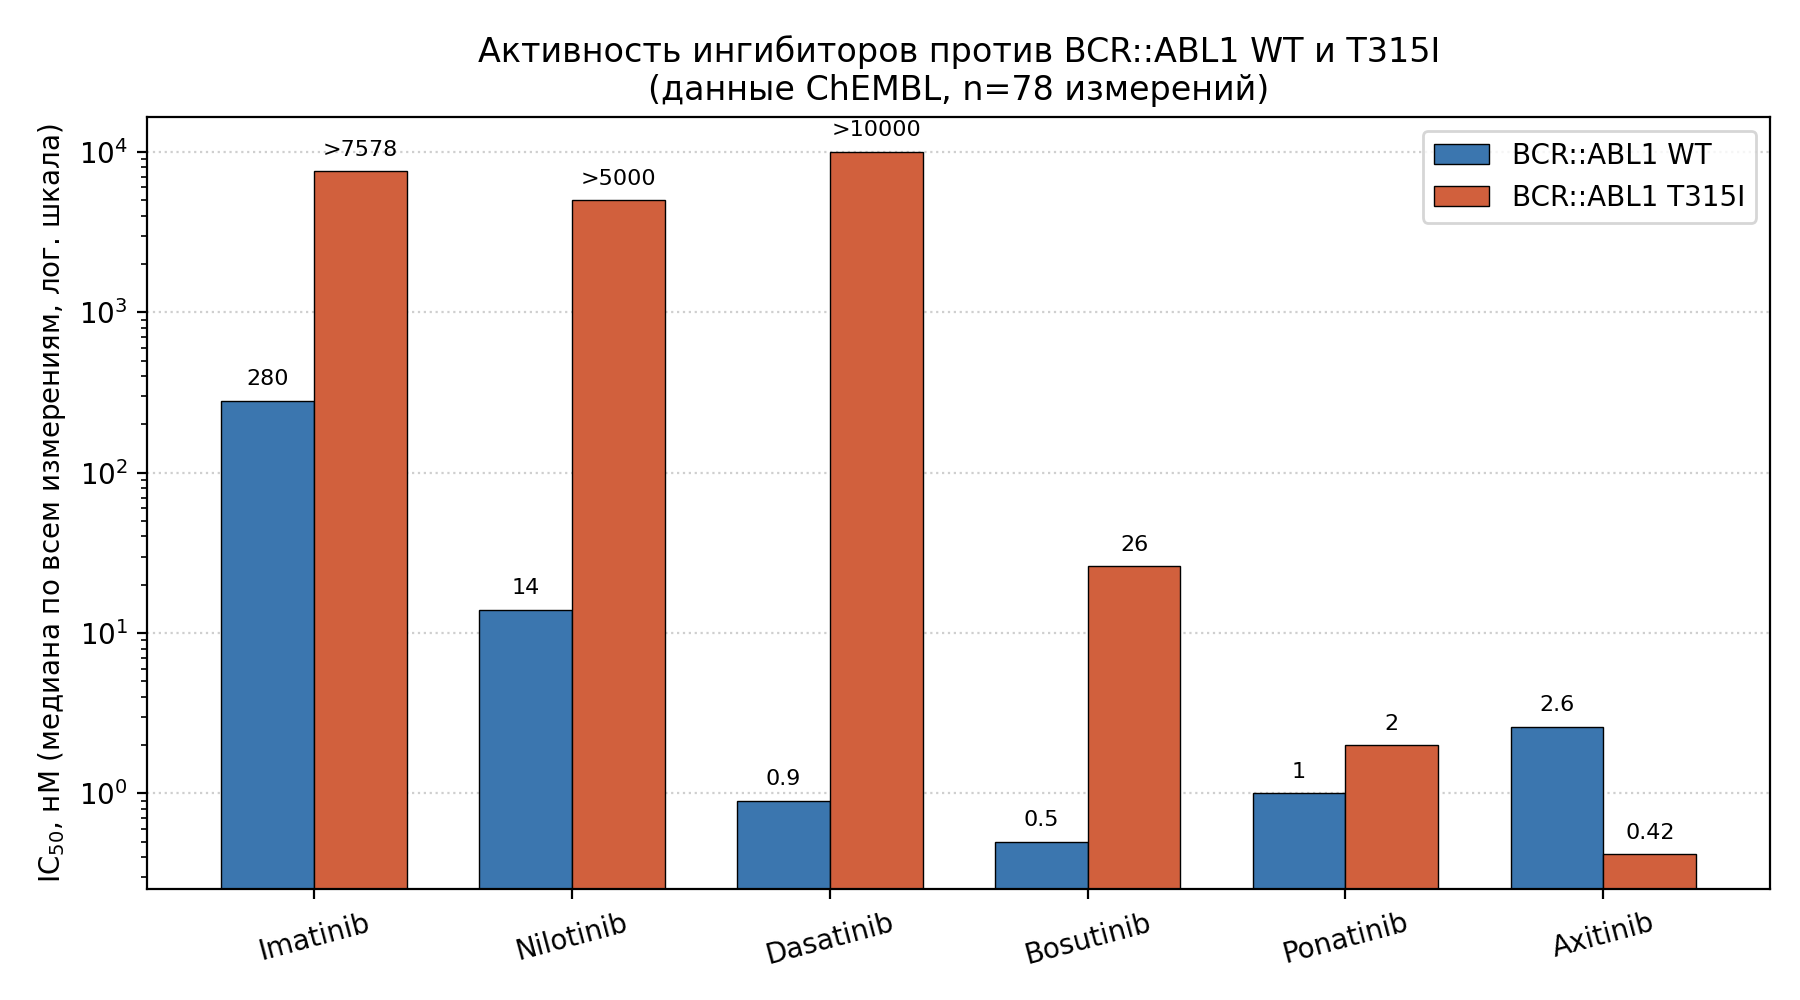
\includegraphics[width=0.95\linewidth]{../figures/fig_activity.png}
\end{figure}

\emph{\small Медианные значения IC$_{50}$ для каждого соединения по всем измерениям из
собранного набора данных; логарифмическая шкала. Знак «$>$» над столбцом означает, что в
число измерений входят цензурированные значения, то есть истинное IC$_{50}$ ещё выше.
Построено скриптом \code{scripts/plot\_activity.py} по файлу
\code{BCR\_ABL\_dataset.csv}.}

\textbf{Краткая интерпретация графика:}

Для ингибиторов 1-го и 2-го поколений (иматиниб, нилотиниб, дазатиниб) переход от WT к
T315I увеличивает IC$_{50}$ на 1--4 порядка: наиболее драматично для дазатиниба, у
которого активность падает с $\approx$0{,}9 нМ до $>10\,000$ нМ. Бозутиниб занимает
промежуточное положение: потеря активности заметная (0{,}5 $\rightarrow$ 26 нМ), но не
катастрофическая, хотя клинически он против T315I всё равно не применяется. У понатиниба
разница между формами составляет менее одного порядка, а у аксетиниба активность против
мутанта даже \emph{выше}, чем против WT --- именно этот эффект стал основанием
рассматривать его как кандидата для перепрофилирования при T315I-резистентности. График
наглядно показывает, что T315I --- не «общее ухудшение связывания», а избирательный
эффект, зависящий от того, опирается ли конкретная молекула на контакт с
gatekeeper-остатком.

\section{Target Data Passport}

\begin{center}
\begin{tabular}{|L{4.3cm}|L{5.4cm}|L{5.4cm}|}
\hline
\textbf{Параметр} & \textbf{BCR::ABL1 WT} & \textbf{BCR::ABL1 T315I} \\
\hline
Исследуемый domain & ABL1 kinase domain, остатки 242--493 (UniProt P00519) &
то же, ABL1 kinase domain 242--493 \\
\hline
Аминокислота 315 & Thr & Ile \\
\hline
PDB structures доступны? & да, 60 записей с киназным доменом &
да, 8 записей (из них 4 --- человеческий ABL1) \\
\hline
Выбранный PDB ID & \textbf{2HYY} & \textbf{3QRJ} \\
\hline
Experimental method & X-ray diffraction & X-ray diffraction \\
\hline
Resolution & 2.40~\AA & 1.82~\AA \\
\hline
Ligand & STI --- иматиниб & 919 --- ребастиниб (DCC-2036) \\
\hline
Известные inhibitors & иматиниб, нилотиниб, дазатиниб, бозутиниб, понатиниб, асциминиб
(все активны) & понатиниб, асциминиб; in~vitro также аксетиниб; TKI 1--2 поколений
неактивны \\
\hline
Activity data доступны? & да: IC$_{50}$ и K$_d$, 42 измерения в собранном наборе &
да, но частично цензурированы ($>5000$, $>10\,000$ нМ), 36 измерений \\
\hline
Достаточно данных для дальнейшего modelling? & да & да, с оговорками (см. раздел~13) \\
\hline
\end{tabular}
\end{center}

\section{Итоговый вывод}
\instr{Ответьте на вопрос: достаточно ли доступных данных по BCR::ABL1 WT и T315I для
дальнейшего computational drug discovery? Отдельно оцените структурные данные, известные
ингибиторы, activity data и наличие машиночитаемых химических структур.}

В целом --- да, обе формы мишени обеспечены данными достаточно, чтобы переходить к
структурному анализу, докингу и хемоинформатике.

\textbf{Структурные данные.} Достаточно. Для киназного домена ABL1 доступно 68 записей
PDB, из них 60 соответствуют форме WT и 8 --- T315I; подавляющее большинство получено
рентгеновской дифракцией с разрешением 1{,}8--2{,}5~\AA. Выбранные структуры 2HYY
(2{,}40~\AA) и 3QRJ (1{,}82~\AA) --- человеческий белок без посторонних мутаций, с
полностью разрешённым сайтом связывания.

\textbf{Данные о лигандах.} Достаточно. Известно как минимум шесть одобренных препаратов
и десятки исследовательских соединений; 64 из 68 структур киназного домена содержат
связанную малую молекулу, то есть доступны экспериментальные позы лигандов --- это
позволит валидировать протокол докинга редокингом.

\textbf{Activity data.} Достаточно, но требует осторожности. Собрано 78 измерений
IC$_{50}$/K$_d$ из 11 первичных источников. Значения разнородны по методике, и для T315I
заметная часть данных цензурирована.

\textbf{Chemical data.} Достаточно. Для всех соединений получены PubChem CID,
брутто-формула, молекулярная масса и SMILES (с учётом стереохимии), то есть данные
полностью машиночитаемы.

\textbf{Обнаруженные ограничения и пробелы в данных:}
\begin{enumerate}[leftmargin=*,topsep=2pt,itemsep=3pt]
\item \textbf{Асимметрия по формам мишени.} Структур T315I в 7{,}5 раза меньше, чем WT
(8 против 60), а человеческих --- всего 4. Для мутанта выбор структуры практически
безальтернативен.
\item \textbf{Нет структуры полноразмерного BCR::ABL1.} Все экспериментальные данные
относятся к изолированному киназному домену ABL1; вклад BCR-части структурно не
охарактеризован.
\item \textbf{Цензурированные значения активности.} Для иматиниба, нилотиниба и
дазатиниба против T315I большинство величин --- это границы ($>5000$, $>10\,000$ нМ).
Для регрессионных моделей (QSAR) такие данные напрямую непригодны.
\item \textbf{Неоднородность анализов.} Разброс IC$_{50}$ одного соединения между
публикациями достигает двух порядков (иматиниб против WT: 75--7700 нМ).
\item \textbf{Пробелы в ChEMBL.} Для асциминиба не нашлось записи активности с явной
пометкой T315I, хотя из литературы известно, что он сохраняет активность против этого
мутанта. Автоматическая выгрузка из базы не заменяет проверку по первичным публикациям.
\item \textbf{Нет AlphaFold-модели мутанта и слитного белка.} Модель T315I при
необходимости придётся строить самостоятельно.
\item \textbf{Разные системы нумерации остатков} (изоформы 1a/1b, мышиный ортолог) ---
источник ошибок при сопоставлении структур и литературных данных.
\end{enumerate}

\textbf{Итог:} накопленных данных достаточно для следующих этапов курса. Для дальнейшей
работы фиксируются структуры \textbf{2HYY (WT)} и \textbf{3QRJ (T315I)} и набор данных
\code{BCR\_ABL\_dataset.csv} (78 измерений, 7 соединений).

\vspace{1.2cm}

\noindent Подпись студента: \underline{\hspace{5cm}} \hfill
Дата: \underline{\hspace{3.5cm}}

\end{document}
